\chapter{Sortering og udvalg}
\vspace*{-4.5cm}
\begin{flushright}
\includegraphics[width=6cm]{img/queue2.eps}
\end{flushright}
\vspace*{1cm}

\renewcommand{\labelprefix}{ch:sort}
\llabel{}
\providecommand{\key}{{\mathit key}}
\index{sortering|textbf}

Sandsynligvis har læseren en intuitiv opfattelse af, hvad \emph{sortering} drejer sig om.
Alligevel vil vi definere opgaven formelt.
Input er en følge $s=\seq{e_1,\ldots,e_n}$ af $n$ indgange.
\index{indgang}
Hver indgang $e_i$ er forsynet med en \emph{nøgle}
\index{nzgle@nøgle}
 $k_i = \Id{key}(e_i)$.
Nøglerne er taget fra et ordnet univers, dvs. at der defineret en \emph{lineær} (også kaldt \emph{total}) ordning $\leq$ (se appendix~\ref{app:notation:}).
\index{ordning!lineær}
\index{ordning!total}
For at holde notationen overskuelig, overfører vi ordningsrelationen fra nøgler til indgange, så vi skriver $e\leq e'$ når vi mener $\Id{key}(e)\leq \Id{key}(e')$.
(Idet forskellige indgange kan have samme nøgle, danner den lineære ordning $\le$ altså en lineær \emph{præ}ordning på indgangene, se appendix~\ref{app:notation:}).
Opgaven består i at skabe en følge $s'=\seq{e'_1,\ldots,e'_n}$, som er en permutation
\index{permutation}
af $s$, så der gælder $e'_1\leq \cdots\leq e'_n$.
Læg mærke til, at rækkefølgen af indgange med samme nøgle er vilkårlig.
\index{sortering|textbf}

Selvom en og samme datatype kan tillade mange forskellige sammenligningrelationer, har visse datatyper en naturlig ordningsrelation:
For tal er dette den sædvanlige ordning.
For tupler, strenge og følger bruges den leksikografiske ordning (se appendix~\ref{app:notation:}).
Den leksikografiske ordning på strenge findes i forskellige udgaver.
Man kan se store og små bogstaver som ens eller forskellige, og i mange sammenhænge behandles bogstaver med accenter eller ligaturer på forskellige måder.

\begin{exerc}
Givet lineære ordninger $\le_A$ på $A$ og $\le_B$ på $B$, definer en lineær ordning på $A \times B$. 
\end{exerc}

% TODO: removed complex number exercise from orig

Sortering er et allestedsnærværende algoritmisk værktøj, som ofte optræder som forberedende skridt
\index{sortering!anvendelse}
\index{algoritmekonstruktion!sortering (anvendelse)}
i mere komplekse algoritmer.
Vi skal se nærmere på nogle eksempler.

\begin{itemize}
\item 
\emph{Forberedelse til hurtig søgning}.
\index{algoritmekonstruktion!forberedelse}
  I afsnit~\ref{ch:intro:s:binary search}, som omhandlede binærsøgning, så vi at søgning i en ordnet telefonbog er lettere at gennemføre, såvel for mennesker som for datamaskiner.
\index{søgning!binærsøgning}
Derudover understøtter en ordnet telefonbog flere operationer som at finde samtlige indgange inden for et område \index{søgning!område}.
Søgning behandles indgående i kap.~\ref{ch:search:}.
For at søge i uordnede mængder kan man også bruge hakning.
 \index{hakning}
\item \emph{Gruppering}.
\index{gruppering}
\index{sortering!anvendelse}
\index{algoritmekonstruktion!sortering (anvendelse)}
Ofte ønsker man at bringe identiske indgange på en og samme plads, måske for at tælle dem, eller for at identificere og fjerne eller håndtere dubletter.
  Også her tilbyder hakning\index{hakning!anvendelse} en alternativ løsning. 
Men sortering byder på flere fordele: vi skal møde hurtige, pladseffektive, deterministiske 
\index{algoritmekonstruktion!deterministisk}
sorteringsmåder, som skalerer til kæmpestore datamængder.
\item \emph{Behandling i sorteret rækkefølge}.
\index{sortering!anvendelse}
\index{algoritmekonstruktion!sortering (anvendelse)}
Mange algoritmer forenkles væsentligt af at behandle input i sorteret rækkefølge.
I opgave~\lref{ex:schedule} finder man et eksempel. 
Andre eksempler er Kruskals algoritme i afsnit~\ref{ch:mst:s:kruskal}  og nogle af algoritmerne for rygsæksproblemet i kap.~\ref{ch:optimization:}.
Det kan også være nyttigt at tænke på sortering, når man prøver at løse opgave~\ref{ch:grepresent:ex:interval} om intervalgrafer \index{graf!intervalgraf}.
\end{itemize}

I afsnit~\lref{s:simple} skal vi præsentere nogle enkle sorteringsalgoritmer.
Deres tidsforbrug er kvadratisk, men de er alligevel brugbare for små problemstørrelser.
Vi skal også se på nogle maskinnære optimeringer.
I afsnit~\lref{s:merge} præsenteres \emph{flettesortering}, en enkel del-og-hersk-algoritme, som har kørselstid $O(n\log n)$.
Som vi skal vise i afsnit~\lref{s:lower}, er denne tidsgrænse optimal for alle \emph{sammenligningsbaserede} sorteringsalgoritmer, dvs. algoritmer, so betragter indgangene som »sorte kasser«, som kan tillader parvis sammenligning og flytning.
\emph{Kviksortering}, som behandles i  afsnit~\lref{s:quick}, beror ligeledes på en del-og-hersk-tilgang.
Måske er den den mest anvendte sorteringsalgoritme.
Kviksortering er et fremragende eksempel på en randomiseret algoritme.
Algoritmens grundlæggende idé fører også til en enkel algoritme for \emph{udvalgsproblemet}:
I afsnit~\lref{s:select} skal vi se, hvordan man kan finde den $k$te-mindste indgang i en mængde af størrelse $n$ i forventet tid $O(n)$.
Når nøgler har en kendt struktur, som fx tal eller talfølger, eller kan behandles som sådan, kan man sortere hurtigere end den nedre grænser fra afsnit~\ref{s:lower}.
Hertil skal nøgler udsættes for andre operationer end sammenligninger, fx ved at udnytte nøglens numeriske repræsentation.
Endelig skal afsnit~\lref{s:external} præsentere meget gode algoritmer på basis af \emph{kviksortering} og \emph{flettesortering}, som tillader sortering af data, som ikke får plads i hovedlageret.

\begin{exerc}[Planlægning: Hotelreservationer]
  \llabel{ex:schedule}
  \index{sortering!anvendelse}
  \index{algoritmekonstruktion!sortering (anvendelse)}
  En hoteldirektør har $n$ reservationer til næste sæson.
  Hotellet har $k$ identiske værelser.
  En reservation består af en ankomstdato og en afrejsedato.
  Hoteldirektøren vil vide, om hotellets værelser er nok til at opfylde alle ønsker.
  Konstruer en algoritme, som efter sortering løser problemet i tid $O(n)$.
  \emph{Vink}: 
  Sorter først (multi-)mængden af alle ankomst- og afrejsetidspunkter.
  Behandl derefter den denne mængde i ét gennemløb i stigende rækkefølge.
\end{exerc}


\begin{exerc}[Sortering med lille nølgemængde]
  \index{hakning!anvendelse}
  Konstruer en algoritme, som sorterer $n$ indgange i forventet tid $O(k\log k + n)$, hvis der kun forekommer $k$ forskellige nøgler i input.
  \emph{Vink}: 
  Anvend et senere resultat i dette kapitel, nemlig at man kan sortere $k$ nøgler i tid $O(k\log k)$. 
  Kombiner hakning og sortering.
\end{exerc}


\begin{exerc}[Resultatkontroll]\llabel{ex:check}\index{algoritmekonstruktion!resultatkontroll}
  Det er nemt at kontrollere, om en sorteringsmåde faktisk har skabt en voksende følge.
  Derimod er det mindre nemt at kontrollere, om den resulterende følge er en permutation af det oprindelige input.
  \index{permutation}
  Hvis nøglerne er heltal, findes der dog en enkel og hurtig Monte Carlo-algoritme
til formålet:
  \index{algoritmekonstruktion!stokastisk!Monte Carlo}
(a)
Vis, at $\seq{e_1,\ldots,e_n}$ er en permutation  af 
$\seq{e'_1,\ldots,e'_n}$, hvis og kun hvis polymomiet $q$ givet ved
  \[ q(x) = \prod_{i=1}^n(x-e_i)-\prod_{i=1}^n(x-e'_i)\]
\index{Polynom}
  er nulpolynomiet. 
  Her er $x$ en variabel.
(b) For givet $\epsilon>0$ lad
$p$ være et primtal
  \index{primtal}
  \index{algoritmekonstruktion!algebraisk} 
  med
  $p>\max\{n/\epsilon,e_1,\ldots,e_n,e'_1,\ldots,e'_n\}$.
  Idéen er nu at evaluere polynomiet foroven modulo $p$ i $x=r$ for en tilfældig værdi
  $r\in\{0,\ldots, p-1\}$. 
  Vis at dersom $\seq{e_1,\ldots,e_n}$ \emph{ikke} er en permutation af  $\seq{e'_1,\ldots,e'_n}$,  så er $q(r)=0$ med sandsynlighed højst $\epsilon$.
\emph{Vink}: Et polynomium af grad højst $n$, som ikke er nulpolynomiet modulo $p$, har højst $n$ rødder, når man regner modulo $p$.
%TODO very clumsy with the modulo
\end{exerc}


%%%%%%%%%%%%%%%%%%%%%%%%%%%%%%%%%%%%%%%%%%%%%%%%%%%%%%%%%%%%%%%%%%%%%%
\section{Enkle sorteringsteknikker}\llabel{s:simple}

Vi præsenterer nu to enkle sorteringsteknikker, \emph{udvalgssortering} og \emph{indsættelsessortering}. 

\index{algoritmekonstruktion!grådig}%
Ved udvalgssortering
\index{sortering!udvalgs-|textbf}
\index{udvalgssortering|sieheunter{sortering}}
gentager man følgende skridt:
Vælg den første indgang i inputfølgen, slet den der, og føj den til outputfølgen.
Outputfølgen er tom til at begynde med;
processen fortsætter, til inputfølgen er tom.
For eksempel,
\[ \seq{\,},\seq{4,7,1,1}\leadsto
\seq{1},\seq{4,7,1}\leadsto
\seq{1,1},\seq{4,7}\leadsto
\seq{1,1,4},\seq{7}\leadsto
\seq{1,1,4,7},\seq{\,}\,. \]
Algoritmen kan implementeres sådan, at den kan nøjes med en enkelt række af $n$ indgange og arbejder \emph{på plads},
\index{sortering!på plads@\emph{på plads}|textbf}
dvs. at den ud over inputrækken og et konstant antal lagerceller for iterationsvariable o. lign. ikke behøver mere plads.
Kørselstiden er kvadratisk.

I afsnit~\ref{ch:pq:s:further}
beskrives en mere raffineret implementation af udvalgssortering, som forvalter inputfølgen som en \emph{prioritetskø}.
\index{prioritetskø!anvendelse}
Prioritetskøen gør det muligt at vælge og fjerne en mindste indgang effektivt.
Det resulterende algoritme har kørselstid $O(n\log n)$ og er meget brugt.
Den er effektiv, deterministisk, arbejder på plads, og inputfølgen kan udvides dynamisk
\index{sortering!dynamisk}
med nye elementer, så længe disse er større end de allerede udtagne.
Den sidste egenskab er af stor betydning for den hændelsesstyret diskret simulering, hvor hændelser behandles i tidslig voksende rækkefølge og en hændelse kan lede til nye hændelser, som skal udføres senere.

Ved udvalgssortering udtages den næste indgang fra inputfølgen med henblik på at bevare løkkeinvarianten,
\index{invariant!løkkeinvariant}
nemlig at output\-følgen er sorteret under hele forløbet.
Ved indsættelsessortering%
\index{sortering!indsættelses-|textbf}
\index{indsættelsessortering|sieheunter{sortering}}
gælder samme løkkeinvariant;
her tager man dog en \emph{vilkårlig} indgang fra input\-følgen og sikrer i stedet, at den anbringes på rette plads i output\-følgen.
For eksempel,
\[
\seq{\,},\seq{4,7,1,1}\leadsto
\seq{4},\seq{7,1,1}\leadsto
\seq{4,7},\seq{1,1}\leadsto
\seq{1,4,7},\seq{1}\leadsto
\seq{1,1,4,7},\seq{\,}\,. \]
Fig.~\lref{alg:insert} viser en implementation af indsættelsessortering, som arbejder på plads i ind- og output\-rækken $a[1..n]$. 
Implementationen realiserer den algoritmiske idé på en oplagt måde, bortset fra et enkelt kneb, som gør det muligt at styre den indre løkke med kun én sammenligning.
Når indgangen $e$, som er den næste at blive indføjet, er mindre end alle tidligere indføjede indgange, kan man den stilles forrest uden videre sammenligninger. 
Ellers passerer man hele den sorterede delfølge fra højre til venstre, så længe der ikke står en indgang, som er større end $e$.
Denne proces må nødvendigvis standse, fordi $a[1]\leq e$.
\index{vogter@\emph{vogter}|siehe{vogterindgang}}
\index{vogterindgang}.   

I værstefald er indsættelsessortering temmelig langsom.
Hvis fx input er sorteret i aftagende orden, bliver hver eneste indgang flyttet hele vejen til plads $a[1]$, hvilket betyder, at den $i$te iteration af den ydre løkke skal flytte $i$ indgange.
Samlet giver dette
\[\sum_{i=2}^n(i-1)=
  -n+\sum_{i=1}^ni=
  \frac{n(n+1)}{2}-n=
  \frac{n(n-1)}{2}=\Omega(n^2)\]
  mange flytninger af indgange (se (\ref{app:notation:eq:sumi})).

\begin{figure}
\begin{tabbing}
~~~~\=~~~~\=~~~~\=\kill
  \Procedure \Id{indsættelsessortering}$($\Declare{$a$}{\Array$[1..n]$ \Of Element}$)$\+\\
  \ForFromTo{i}{2}{n}\+\\
    \Invariant $a[1]\leq\cdots\leq a[i-1]$\\
    \comment{sæt $a[i]$ på rette plads}\\
    $e \Is a[i]$\\
    \If $e<a[1]$ \Then\+\comment{nyt minimum}\\
      \ForFromDownto{j}{i}{2} $a[j] \Is a[j-1]$\\
      $a[1] \Is e$ \- \\ 
    \Else\+\comment{anvend $a[1]$ som vogterindgang}\\ 
      \ForFromdownWhile{j}{i}{a[j-1]>e} $a[j] \Is a[j-1]$\\
      $a[j] \Is e$
\end{tabbing}
\caption{\llabel{alg:insert}Indsættelsessortering.}
\end{figure}

På trods af den dårlige værstefaldsopførsel er indsættelsessortering en nyttig metode.
Den er hurtig for små input
\index{sortering!små input}
(fx $n\le 10$) og kan derfor bruges i bunden af del-og-hersk-algoritmer for sorteringsproblemet.
Desuden er input i mange anvendelsesområder i forvejen allerede »næsten sorteret« 
\index{sortering!næsten sorteret input};
i disse siutationen er indsættelsessortering hurtig.

\begin{exerc}[Næsten sorteret input]\llabel{ex:almost-sorted}
  Vis, at indsættelsessortering har kørselstid $O(n + D)$ med
 $D= \sum_i \left|r(e_i)-i\right|$, hvor
  $r(e_i)$ er \emph{rangen}\index{rang (i sorteret orden)} (dvs. positionen) af $e_i$ i det sorterede output.
\end{exerc}

\begin{exerc}[Gennemsnitsanalyse]\llabel{ex:average-insertion}%
\index{algoritmeanalyse!gennemsnitligt fald}
  Betragt mængden af alle $n!$ mange input, som består af permutationer af tallene fra 
  $1$ til $n$.
  Vis, at den gennemsnitlige kørselstid for indsættelsessortering på disse input er 
  $\Omega(n^2)$.
  \emph{Vink}:
  Vis, at der i gennemsnit en tredjedel af alle de indgange, der står i den oprindelige rækkes højre tredjedel, skal flyttes til rækkens venstre tredjedel.
  Kan du finde et bedre bevis, som desuden viser, at der i gennemsnit kræves
  $\frac{1}{4}n^2-O(n)$ gennemløb af den indre løkke?
\end{exerc}


\begin{exerc}[indsættelsessortering med få sammenligninger]
  Modificer den indre løkke af den rækkebaserede indsættelsessorteringsalgoritme i fig.~\lref{alg:insert}, så den kun behøver $O(n\log n)$ sammenligninger mellem indgange. 
  \emph{Vink}: Binærsøgning, se afsnit~\ref{ch:intro:s:binary search}.
  Hvad er kørselstiden af denne variant?    
\end{exerc}

\begin{exerc}[Effektiv indsættelsessortering?]
  Brug datastrukturen for ordnede følger fra kap.~\ref{ch:search:} for at skabe en variant af indsættelsessortering med kørselstid $O(n\log n)$. 
\end{exerc}

\begin{exerc}[Formel verifikation]\index{verifikation}
  Brug din foretrukne verifikationsformalisme (fx hoarelogik) for at vise formelt, at indsættelsessortering producerer en permutation af inputfølgen.
\end{exerc}

\section{Flettesortering}
\llabel{s:merge}%
\index{sortering!flette-|textbf}%
\index{flettesortering|sieheunter{sortering}}%
\index{algoritmekonstruktion!del-og-hersk!flettesortering}

Flettesortering eller en enkel og direkte anvendelse af del-og-hersk-princippet
Den usorterede følge deles op i to omtrent lige store dele.
Begge dele sorteres rekursivt, hvorefter begge delfølger flettes sammen til én ordnet følge.
Denne tilgang er effektiv, fordi fletningen af to ordnede følger $a$ og $b$ kan gøres enkelt og hurtigt.
Den mindste indgang for begge følger er enten den første indgang i $a$ eller den første indgang i $b$.
Vi flytter denne mindste indgang til output\-følgen, fortsætter med at finde den næstmindste indgang, osv.
Processen gentages, indtil alle indgange er vandret over i output.
I fig.~\lref{alg:mergesort} vises algoritmen i pseudokode, og i fig.~\lref{fig:mergesort} vises et eksempel på en kørsel på konkret input.
Hvis de indgående følger er (enkelt-)hægtede lister (se afs.~\ref{ch:sequence:ss:slist}), behøves hverken reservation eller frigørelse af listeindgange.
Hver iteration i den indre løkke af proceduren \Id{flet} fører til én sammenligning af indgange og flytter én ingang til outputfølgen; dette kan gøres i konstant tid.
Derfor er kørselstiden for fletning lineær.

\begin{figure}
  \begin{tabbing}
    ~~~~\=~~~~\=\kill
    \Funct{flettesorter}{$\seq{e_1,\ldots,e_n}$}{\Id{Følge}\ \Of \Id{Element}}\+\\
  \If $n=1$ \Then \Return $\seq{e_1}$ \\ 
  \Else \Return \Id{flet}(\,\=\Id{flettesorter}$(\seq{e_1,\ldots,e_{\floor{n/2}}}),$\\
                        \>$\Id{flettesorter}(\seq{e_{\floor{n/2}+1},\ldots, e_n})\,)$\-\\[2mm]

\comment{Flet to ordnede følger, repræsenteret som lister}\\
~~~~\=~~~~\=\kill
    \Funct{flet}{\Declare{$a,b$}{\Id{Følge}\ \Of \Id{Element}}}{\Id{Følge}\ \Of \Id{Element}}\+\\
  $c\Is\seq{\,}$\\ 
  \Loop\+\\
    \Invariant både $a$, $b$ og $c$ er i stigende ordning og $\forall e\in c, e'\in a\cup b\colon e\leq e'$\\
    \If $a.\Id{første}\leq b.\Id{første}$ \=\kill
    \If $a.\Id{tom}$\>\Then $c.\Id{sammenføj}(b)$; \Return c \\
    \If $b.\Id{tom}$\>\Then $c.\Id{sammenføj}(a)$; \Return c  \\
    \If $a.\Id{første}\leq b.\Id{første}$  \>\Then\=
    $c.\Id{flytTilBagest}(a.\Id{første})$\\
    \Else \>\>$c.\Id{flytTilBagest}(b.\Id{første})$
\end{tabbing}
    \caption{\llabel{alg:mergesort}Flettesortering.}
\end{figure}

\begin{figure}[t]
  \small
\begin{minipage}{0.4\textwidth}
  \begin{tikzpicture}[scale =.5,
    s/.style = {font = \small, inner sep = 0pt}]
    \node (2718281) at (-.5,0)  [s] {$\seq{2,7,1,8,2,8,1}$};
    \node (1122788) at (-.5,-6) [s] {$\seq{1,1,2,2,7,8,8}$};
    \node (271)     at (-2.5,-1)[s] {$\seq{2,7,1}$};
    \node (127)     at (-2.5,-5)[s] {$\seq{1,2,7}$};
    \node (2)       at (1,-3)   [s] {$\seq{2}$};
    \node (2u)      at (-3.5,-2)[s] {$\seq{2}$};
    \node (71)      at (-1.5,-2)[s] {$\seq{7,1}$};
    \node (17)      at (-1.5,-4)[s] {$\seq{1,7}$};
    \node (7)       at (-2,-3)  [s] {$\seq{7}$};
    \node (8281)    at (1.5,-1) [s] {$\seq{8,2,8,1}$};
    \node (1288)    at (1.5,-5) [s] {$\seq{1,2,8,8}$};
    \node (81)      at (2.5,-2) [s] {$\seq{8,1}$};
    \node (18)      at (2.5,-4) [s] {$\seq{1,8}$};
    \node (1a)       at (-1,-3) [s] {$\seq{1}$};
    \node (1b)       at (3,-3)  [s] {$\seq{1}$};
    \node (8a)      at (0, -3)  [s] {$\seq{8}$};
    \node (8b)      at (2,-3)   [s] {$\seq{8}$};
    \node (82)      at (0.5,-2) [s] {$\seq{8,2}$};
    \node (28)      at (0.5,-4) [s] {$\seq{2,8}$};
    \node at (-5,-0.5) {del};
    \node at (-5,-1.5) {del};
    \node at (-5,-2.5) {del};
    \node at (-5,-3.5) {flet};
    \node at (-5,-4.5) {flet};
    \node at (-5,-5.5) {flet};
    \draw [callout] (2718281) -- (271);
    \draw [callout] (2718281) -- (8281);
    \draw [callout] (271) -- (2u);
    \draw [callout] (271) -- (71);
    \draw [callout] (8281) -- (82);
    \draw [callout] (8281) -- (81);
    \draw [callout] (71) -- (7);
    \draw [callout] (71) -- (1a);
    \draw [callout] (82) -- (8a);
    \draw [callout] (82) -- (2);
    \draw [callout] (81) -- (8b);
    \draw [callout] (81) -- (1b);
    \draw [callout] (8a) -- (28);
    \draw [callout] (2) -- (28);
    \draw [callout] (7) -- (17);
    \draw [callout] (1a) -- (17);
    \draw [callout] (8b) -- (18);
    \draw [callout] (1b) -- (18);
    \draw [callout] (2u) -- (127);
    \draw [callout] (17) -- (127);
    \draw [callout] (28) -- (1288);
    \draw [callout] (18) -- (1288);
    \draw [callout] (127) -- (1122788);
    \draw [callout] (1288) -- (1122788);
  \end{tikzpicture}
\end{minipage}
\begin{minipage}{0.55\textwidth}
\begin{flushright}%
\begin{tabular}{rrll}
$a$ & $b$ & $c$ & Operation\\\midrule
$\seq{1,2,7}$ &$\seq{1,2,8,8}$ &  $\seq{\,}$ & flyt fra $a$\\
$\seq{2,7}$ &$\seq{1,2,8,8}$ &  $\seq{1}$ & flyt fra $b$\\
$\seq{2,7}$ &$\seq{2,8,8}$ &  $\seq{1,1}$ & flyt fra $a$\\
$\seq{7}$ &$\seq{2,8,8}$ &  $\seq{1,1,2}$ & flyt fra $b$\\
$\seq{7}$ &$\seq{8,8}$ &  $\seq{1,1,2,2}$ & flyt fra $a$\\
$\seq{\,}$ &$\seq{8,8}$ &  $\seq{1,1,2,2,7}$ & sammenføj $b$\\\midrule
$\seq{\,}$ &$\seq{\,}$ &  $\seq{1,1,2,2,7,8,8}$ & \\
\end{tabular}
\end{flushright}%
\end{minipage}
\caption{
  \llabel{fig:mergesort}
  Kørsel af
  $\Id{flettesorter}(\seq{2,7,1,8,2,8,1})$.
  \emph{Til venstre} vises strukturen af de rekursive kald i
  \index{algoritmekonstruktion!rekursion}
  i $\Id{flettesorter}$.
  \emph{Til højre} vises kørslen af $\Id{flet}$ i det yderste kald.}
\end{figure}

\begin{thm}\llabel{thm:merge}
Proceduren \Id{flet} anvendt på to følger af samlet længde $n$ udføres i tid $O(n)$ og bruger højst $n-1$ sammenligninger af indgange.
\end{thm}

For kørselstiden af flettesortering får vi følgende:

\begin{thm}\llabel{thm:mergesort}
  Flettesortering af en følge af længde $n$ udføres i tid $O(n\log n)$ og bruger højst $\floor{n\log n}$ sammenligninger af indgange.
  %TODO n undefined in orig
\end{thm}

\begin{proof}
  Lad $C(n)$ være antallet af sammenligninger, som i værste fald gennemføres på en inputfølge af $n$ indgange.
  Åbenbart er $C(1)=0$, og fra sætning~\lref{thm:merge} får vi $C(n) \le C(\floor{n/2})+C(\ceil{n/2})+n-1$.
  Hovedsætningen for rekursionsligninger (sætning~\ref{ch:intro:thm:master})
  \index{algoritmeanalyse!hovedsætning}
  \index{algoritmeanalyse!rekursion}
  giver da $C(n) = O(n \log n)$.
  Vi skal nu give to direkte beviser, som leverer eksplicitte konstanter.
  Det første bevis etablerer $C(n) \le 2n \ceil{\log n}$, det andet sågar $C(n) \le n \log n$.

 Hvis $n$  er en 2-potens, definerer vi $D(1) = 0$ og $D(n) = 2D(n/2) + n$. 
 Et enkelt induktionsbevis viser, under anvendelse af ligningen $\log(n/2)=\log n - 1$, 
 at der gælder $D(n) = n \log n$ når $n$ er en topotens.
 Lad nu $n$ være vilkårlig.
  Vi betragter det entydigt bestemte $k$, som opfylder $2^{k-1} < n \le 2^k$, og påstår, at der gælder $C(n) \le D(2^k)$.
  Heraf følger direkte
 $C(n) \le D(2^k) = 2^k\cdot k \le 2n \ceil{\log n}$. 
 Uligheden $C(n) \le D(2^k)$ viser vi ved induktion efter $k$. 
 For $k = 0$ gælder $n = 1$ og $C(1) = 0 = D(1) = D(2^0)$.
 For $k > 1$ indser vi først, at der gælder $\floor{n/2} \le \ceil{n/2} \le 2^{k-1} < n$.
 Ved at anvende rekursionsligningen og induktionsantagelsen får vi nu uligheden
 \[ C(n) \le C(\floor{n/2})+C(\ceil{n/2})+n-1 \le 2D(2^{k-1}) + 2^k - 1 \le
 D(2^k)\,. \] 
 Det afslutter det første bevis.

 Vi vender os nu mod den andet, mere nøjeregnende bevis, hvor vi vil etablere grænsen
 \[ C(n)\leq n\ceil{\log n}-2^{\ceil{\log n}} + 1 \] 
 ved induktion efter $n$. 
 For $n = 1$ gælder påstanden åbenbart. 
 Antag altså $n>1$.
 Betragt det $k$, som opfylder $2^{k-1}<\ceil{n/2}\le 2^k$, dvs. $k = \ceil{\log(\ceil{n/2})}$.
 Så gælder ifølge induktionshypotesen, at $C(\ceil{n/2})\le \ceil{n/2}k -2^k + 1$.
 For $2^{k-1} < \floor{n/2}$ følger ligeledes af induktionshypotesen, at $C(\floor{n/2})\le \floor{n/2}k -2^k + 1$.
 For $\floor{n/2}=2^{k-1}$ giver induktionshypotesen, at
 $C(\floor{n/2})\le \floor{n/2}(k-1) -2^{k-1} + 1$.
 Men højresiden er lig med
 $2^{k-1}\cdot(k-1) -2^{k-1} + 1 = 2^{k-1}\cdot k -2^k+1=\floor{n/2}k -2^k + 1$.
 Vi får altså i hvert fald:
 \begin{align*}
   C(n) &\leq C(\floor{n/2})+C(\ceil{n/2})+n-1 \\
   &\le \big(\floor{n/2} k -2^k + 1\big)+ \big(\ceil{n/2}k -2^k + 1\big) + n - 1 \\
   & =  n k + n - 2^{k+1} + 1 = n(k+1) - 2^{k+1} + 1 = n\ceil{\log
   n}-2^{\ceil{\log n}} + 1 \,.
 \end{align*}
 Nu skal vi vise, at 
  $k=\ceil{\log n}$ opfylder uligheden $nk-2^k + 1 \le n\log n$.
 For $n=2^k$ gælder $2^k\cdot k - 2^k + 1\le 2^k\cdot k$ åbenbart. 
 For $n<2^k$ indser vi $nk-2^k+1 \le n(k-1) + (n-2^k+1) \le n\log n$.

 Grænsen for kørselstiden etableres med en lignende rekursionsligning
 (jf. opgave~\ref{ch:intro:ex:mergesortrecurrence}).
\end{proof}

Flettesortering er den foretrukne metode for at sortere hægtede lister.
\index{liste!sortering}
\index{sortering!liste}
Derfor bruges denne fremgangsmåde ofte i funktions- og logikprogrammeringssprog,
\index{programmeringssprog!funktions-}
\index{programmeringssprog!logik-} 
idet disse sprog bruger lister som den primære datastruktur.
I afsnit~\lref{s:lower} skal vi se, at flettesortering i grunden er optimal med hensyn til antallet af sammenligninger.
Derfor er det også et godt valg, når sammenligninger er dyre. 
Ved implementationen baseret på rækker har flettesortering desuden den fordel, at den gennemgår lagerafsnit sekventielt. 
Det fører til effektivitetsforedele i situationer med et lagerhierarki; mere om dette emne i afsnit~\lref{s:external}.
Alligevel er flettesortering ikke det foretrukne metode til at sortere rækker, fordi \Id{flet} ikke arbejder på plads, men behøver yderligere lager.
(En mulig udvej betragtes i opgave~\lref{ex:blockmerge}.)


\begin{exerc}
  Forklar, hvordan man føjer $k$ nye indgange til en ordnet liste i tid $O(k\log k +n)$.
  \index{liste!massetilføjelse|textbf}
\end{exerc}

\begin{exerc}
  Fig.~\lref{alg:mergesort} beskriver proceduren $\Id{flet}$ for lister, men $\Id{flettesortering}$ bare i abstrakt følgeterminologi. 
  Beskriv $\Id{flettesortering}$ detaljeret for hægtede lister. 
\end{exerc}

\begin{exerc}
  Implementer flettesortering i et funktionsprogrammeringssprog.
  \index{programmeringssprog!funktions-}
\end{exerc}


\begin{exerc}
  Implementer flettesortering for rækker i dit foretrukne imperative programmeringssprog.
  Ved siden af inputrækken bruger man en hjælperække af størrelse $n$; de to rækker skiftes til at indeholde mellemresultater og outputfølgen under opbygning.
  Afgør eksperimentelt, om  den faktiske kørselstid bliver bedre ved at skifte fra rekursion til indsættelsessortering for små input.
  \index{sortering!indsættelses-} 
  I så fald, ved hvilken længde er det bedst at skifte?
\end{exerc}

\begin{exerc}
  I vores beskrivelse af \Id{flet} indeholder hvert løkkegennemløb tre sammenligninger -- en sammenligning af indgange og to tomhedstest for løkkeafslutning.
  %TODO
  Udvikl en variant, som i stedet benytter vogterindgange
  \index{vogterindgang} 
  og derved klarer sig med kun én test for løkkeafslutning.
  Går det uden brug af attrapknuder i enden af listen?
\end{exerc}

\begin{exerc}\llabel{ex:blockmerge}
  I opgave~\ref{ch:sequence:ex:blocklist}
  beskrives en repræsentation af følger som en liste af rækker kaldt »blokke«.
  \index{Liste!von Arrays}
  Implementer fletning og flettesortering for denne datastruktur.
  Under fletningen bør tomme inputblokke genbruges til output.
  Sammenlign flettesorterings tids- og pladsbehov for denne datastruktur, for enkelthægtede lister og for rækker, også under hensyntagen til konstante faktorer.
\end{exerc}

\section{En nedre grænse}
\llabel{s:lower}
\index{nedre grænse!sortering|textbf}

Algoritmer giver øvre grænser på problemers beregningskompleksitet.
På baggrund af diskussionen i sidste afsnit ved vi, at $n$ objekter kan sorteres i tid $O(n \log n)$.
Kan det gøres hurtigere -- måske helt ned til lineær tid?
Hvis svaret skulle være »ja«, burde vi kunne fremvise en bedre algoritme og dens analyse.
Men hvordan skulle vi kunne begrunde svaret »nej«?
Vi skulle jo bevise at ingen algoritme, nok så genial, kan sortere i tid $o(n \log n)$.
Sådan et bevis kaldes en \emph{nedregrænse}.
Og hvad er nu svaret? 
Svaret er såvel »ja« som »nej«.
Det er »nej«, hvis vi holder os til sammenligningsbaserede algoritmer,
\index{sammenligningsbaseret algoritme}
og det er »ja«, hvis vi tillader andre slags algoritmer.
Sorteringsmåder, som ikke er baserede på sammenligninger, behandles i afsnit~\lref{s:integer}.
   
Men hvad er egentlig en sammenligningsbaseret sorteringsalgoritme?
Input er en mængde $\set{e_1,\ldots,e_n}$ af $n$ indgange, og algoritmen må ikke gøre andet med disse indgange end parvise sammenligninger og flytninger.
Den eneste måde, at få information om indgange, er at sammenligne dem med hinanden.
Især har algoritmen ikke lov til at benytte nøglens repræsentation, fx som bitstreng.
Til sidste leverer algoritmen en outputfølge $s=\seq{e_1',\ldots,e_n'}$, som er en permutation af inputfølgen og opfylder $e_1'\le\cdots\le e_n'$.
Deterministiske sammenligningsbaserede algoritmer kan man opfatte som træer, kaldt sammenligningstræer.
\index{træ!sammenlignings-|textbf}
Dette indses på følgende måde.
Vejene i træet repræsenterer de forskellige beregninger, hvor træets indre knuder svarer til sammenligninger, og en yderligere knude i slutningen af beregningen svarer til output.
Idet beslutninger i beregningen kun kan være baserede på nøglesammenligninger, kan vejene kun forgrene sig i sammenligningsknuder.
Det springende punkt er, at hvilken sammenligning der udføres hernæst \emph{udelukkende} afhænger af resultatet af de tidligere sammenligninger. 
Figur~\lref{fig:sorttree} viser et sammenligningstræ for tre indgange.

\begin{figure}[b] 
  \newcommand{\compr}{\,{\scriptstyle ?}\,}
  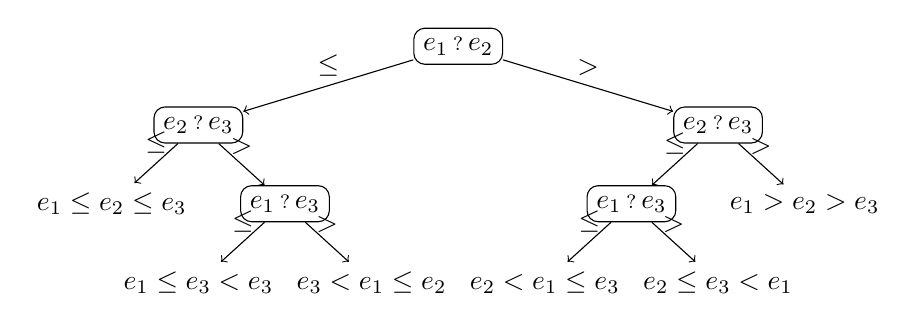
\begin{tikzpicture}[xscale = 1.1]
    \tikzstyle{comp} = [rectangle, draw, rounded corners];
    \node (12) at (0,0) [comp] {$e_1 \compr e_2$};
    \node (23) at (-3,-1) [comp] {$e_2 \compr e_3$};
    \node (23b) at (3,-1) [comp] {$e_2 \compr e_3$};
    \node (13) at (-2,-2) [comp] {$e_1 \compr e_3$};
    \node (13b) at (2,-2) [comp] {$e_1 \compr e_3$};
    \node (ww) at (-4,-2) {$e_1\leq e_2\leq e_3$};
    \node (1w3s2) at (-3,-3) {$e_1\leq e_3< e_3$};
    \node (3s1w2) at (-1,-3) {$e_3< e_1\leq e_2$};
    \node (2s1w3) at (1,-3) {$e_2< e_1\leq e_3$};
    \node (2w3s1) at (3,-3) {$e_2\leq e_3< e_1$};
    \node (1g2g3) at (4,-2) {$e_1> e_2> e_3$};
    \draw [->] (12) to node [above] {$\leq$} (23);
    \draw [->] (23) to node [above] {$\leq$} (ww);
    \draw [->] (12) to node [above] {$>$} (23b);
    \draw [->] (23) to node [above] {$>$} (13);
    \draw [->] (13) to node [above] {$\leq$} (1w3s2);
    \draw [->] (13) to node [above] {$>$} (3s1w2);
    \draw [->] (13b) to node [above] {$\leq$} (2s1w3);
    \draw [->] (13b) to node [above] {$>$} (2w3s1);
    \draw [->] (23b) to node [above] {$\leq$} (13b);
    \draw [->] (23b) to node [above] {$>$} (1g2g3);
  \end{tikzpicture}
\caption{
  \llabel{fig:sorttree}
  Et træ til sortering af tre indgange.
  Først sammenligner vi $e_1$ med $e_2$. 
   Hvis $e_1 \le e_2$, sammenligner vi $e_2$ med $e_3$. 
Hvis $e_2 \le e_3$, så gælder $e_1 \le e_2 \le e_3$, og vi er færdige.
I modsat fald sammenligner vi $e_1$ med $e_3$. 
For hvert af de to mulige resultater er vi færdige.
Hvis $e_1 > e_2$, så sammenligner vi $e_2$ med $e_3$. 
  Hvis $e_2 > e_3$, så har vi $e_1 > e_2 > e_3$ og er færdige. 
  Ellers sammenligner vi $e_1$ med $e_3$. 
  Begge mulige resultater afslutter sorteringen.
  I værste fald sker der tre sammenligninger.
  Det gennemsnitlige antal sammenligninger over alle seks mulige opstillinger er $\frac16(2 + 3 + 3 + 2 + 3 + 3) = \frac83$.}
\end{figure}

Når algoritmen standser, må den have høstet så meget information om input, så den kan lægge sig fast på en permutation 
\index{permutation} 
$\pi$ så input\-indgangene i rækkefølgen $(e_{\pi(1)}, \ldots ,e_{\pi(n)})$ er sorterede.
Hvornår kan algoritmen lægge sig fast?
For at forstå dette, hjælper følgende tankeeksperiment.
Antag, at input\-nøglerne alle er forskellige og betragt hver af de $n!$ mange  permutationer $\pi$ af mængden $\{1,\ldots,n\}$. 
Permutationen $\pi$ svarer til situationen $e_{\pi(1)} < e_{\pi(2)} < \cdots < e_{\pi(n)}$.
For vilkårligt $\pi$ kan vi nu udføre algoritmen og besvare alle den sammenligninger i overensstemmelse med denne rækkefølge.
Dette leder til et blad i sammenligningstræet, som vi kalder $\ell_\pi$.

\begin{lemma} 
  Givet et naturligt tal $n$, en sorteringsalgoritme og det tilhørende sammenligningstræ for input af længde $n$.
  %TODO added quantification of n (comp. trees are nonuniform)
  For to forskellige permutationer $\pi$ og $\sigma$ af $\{1,\ldots, n\}$ er bladene $\ell_\pi$ og $\ell_\sigma$ forskellige.
\end{lemma}

\begin{proof}
  Antag modsætningsvist, at $\pi$ og $\sigma$ er forskellige, men $\ell_\pi$ og $\ell_\sigma$ er ens.
  Betragt to inputfølger $(e_1,\ldots,e_n)$ og $(e_1',\ldots,e_n')$ med $e_{\pi(1)} <  \ldots < e_{\pi(n)}$ og $e'_{\sigma(1)} <  \ldots < e'_{\sigma(n)}$.
  Hver af dem leder til samme blad i sammenligningstræet; dvs. at algoritmen foretager samme omflytning for hver.
  Men så må mindst en af følgende blive fejlsorteret, hvilket er en modstrid med at algortimen er en sorteringsalgoritme.
\end{proof}

Lemmaet medører, at hvert sammenligningstræ, som svarer til en sorteringsalgoritme, skal have mindste $n!$ blade, ét for hvert permutation.
%TODO added clarification "one for each permutation"
Idet et binærtræ af dybde $T$ har højst $2^T$ blade, må der gælde
\[ 2^T \ge n!  \quad\text{og derfor}\quad T \ge \log n!\,.  \]
Fra en enkel nedre grænse (\ref{app:notation:eq:factorial}) på $n!$ fås da
\[ T\geq \log n!\geq \log \left(\left(\frac{n}{e}\right)^n\right)=n\log n - n\log e \,.\]
Vi sammenfatter dette i følgende sætning:

\begin{thm}
  \llabel{thm:lower}
  Hver sammenligningsbaserede sorteringsalgoritme bruger $n\log n-O(n)$ sammenligninger i værste fald.
\end{thm}

Vi nævner uden bevis, grænsen også gælder for randomiserede sorteringsalgoritmer 
\index{algoritmenanalyse!randomiseret}%
\index{algoritmenanalyse!gennemsnitlig}%
samt for det gennemsnitlige tilfælde, hvor alle permutationer af input\-objekterne optræder med samme sandsynlighed.
Grænsen gælder til og med for problemet at afgøre, om input\-følgen indeholder en dublet, hvilket jo umiddelbart virker som en nemmere problem.

For næste sætning går vi ud fra, at input\-følgen består af $n$ forskellige nøgler, og at hver permutation har samme sandsynlighed $1/n!$ for at sortere input\-følgen.

\begin{thm}
  \llabel{thm:lower:average}
  Hver sammenligningsbaserede sorteringsalgoritme bruger i gennemsnit $n\log n-O(n)$ 
  sammenligninger, dvs.
  \[ \frac{\sum_\pi d_\pi}{n!} = n\log n-O(n) \,, \]
  hvor summen er over alle $n!$ permutationer $\pi$ af mængden $\{1,\ldots,n\}$, 
  og $d_\pi$ er dybden af bladet $\ell_\pi$. 
\end{thm}

\begin{exerc}[Sammenligningsbaseret minimum]
  [TODO]
\end{exerc}

\begin{exerc}
  \emph{Unikat}-problemet
  \index{nedre grænse!unikatproblemet|textbf}
  er at afgøre, om elementerne i en givet følge af $n$ indgange med nøgler fra en mængde med total ordning alle er forskellige. 
  Vis, at en sammenligningsbaseret algoritme for dette problem behøver
  $\Omega(n \log n)$ sammenligninger. 
  Hvorfor står dette ikke i modstrid med det faktum, at unikatproblemet kan løses i forventet lineær tid med hakning?
  \index{Hashing!Anwendung}
\end{exerc}

\begin{exerc}[Nedre grænse for det gennemsnitlige tilfælde]
  \llabel{ex:lower:average} 
  [TODO]
\end{exerc}

\begin{exerc}[Optimal sortering af få indgange]
  \index{sortering!få indgange}
  [TODO]
\end{exerc}

\section{Kviksortering}
\llabel{s:quick}
\index{sortering!kvik-|textbf}
\index{kviksortering|sieheunter{sortering}}%

Kviksortering er en del-og-hersk-algoritme
\index{algoritmekonstruktion!del-og-hersk!kviksortering},
som på en vis måde er komplementær til flettesortering fra afsnit~\lref{s:merge}.
Kviksortering udfører broderparten af sit arbejde \emph{inden} de rekursive kald.
Ideen er at placere de givne indgange i en eller flere følger på en sådan måde, at de tilsvarende nøgleområder ikke overlapper hinanden.
I så fald er det nok, at sortere delfølgerne rekursivt \index{algoritmekonstruktion!rekursion}
og sammenføje resultaterne.
For at opnå en fuldkommen dualitet til flettesortering, også i analysen, skulle vi opdele input\-følgen i to følger af eksakt samme længde.
Desværre er dette ikke ligetil.
Vi kan dog komme i nærheden af dette ideal ved at vælge en tilfældig indgang, som vi bruger til at dele følgen i to.
Denne indgang kalder vi \emph{spaltenøgle}.
\index{spaltenøgle|textbf}.
Lad $p$ betegne den valgte spaltenøgle.
Indgangende inddeles nu efter, om de er større, lig med eller mindre end $p$.
Disse tre dele af input organiseres som hver sin følge.
Figur~\lref{alg:quicksort} viser denne ide skematisk, mens figur~\lref{fig:quicksort} viser forløbet på et eksempelinput. 
Kviksortering har forventet kørselstid
\index{algoritmekonstruktion!stokastisk!Las Vegas} 
$O(n\log n)$, hvilket vi skal vise i afsnit~\lref{ss:analysis}.
I afsnit~\lref{ss:refinements} diskuterer vi forbedringer af implementationen, som gør kviksortering til den i praksis mestbenyttede sorteringsalgoritme.
\index{sammenligning!trevejs-}

\begin{figure}
  \begin{tabbing}
    ~~~~\=~~~~\~====\=\kill
\Funct{kviksorter}{\Declare{s}{Følge \Of Element}}{Følge \Of Element}\+\\
  \If $\abs{s}\leq 1$ \Then \Return $s$\quad\comment{Basis}\\
  vælg $p\in s$ tilfældigt\quad\comment{Spaltenøgle}\\
  $a \Is \langle\, e\in s\colon e < p\rangle$\\ %$\RRem{(A)}\\
  $b \Is \langle\, e\in s\colon e = p\rangle$\\ %\RRem{(B)}\\
  $c \Is \langle\, e\in s\colon e > p\rangle$\\ %\RRem{(C)}\\
  \Return sammenføjningen af $\Id{kviksorter}(a)$, $b$ og $\Id{kviksorter}(c)$
\end{tabbing}
  \caption{
    \llabel{alg:quicksort}
    Skematisk fremstilling af kviksortering af lister.}
\end{figure}

\begin{figure}
  \begin{tikzpicture}[
      xscale = .5, 
      yscale  = .75,
      every node/.style = {inner sep = 1pt}
    ]
  \node (3-9) at (4,2) {$\seq{3, 6, 8, 1, 0, 7, 2, 4, 5, 9}$};
  \node (102) at (1,1) { $\seq{1, 0, 2}$};
   \node (0) at (0, 0)  {$\seq{0}$};
   \node (1) at (1, 0)  {$\seq{1}$};
   \node (2) at (2, 0)  {$\seq{2}$};
   \node (3) at (3,1)  {$\seq{3}$};
   \node (e) at (4, -1)  {$\seq{\,}$};
   \node (4) at (5, -1)  {$\seq{4}$};
   \node (5) at (6, -1)  {$\seq{5}$};
   \node (6) at (7,  0)  {$\seq{6}$};
   \node (7) at (8, -1)  {$\seq{7}$};
   \node (8) at (9, -1)  {$\seq{8}$};
   \node (9) at (10,-1)  {$\seq{9}$};
   \node (6-9) at (7,1) {$\seq{6, 8, 7, 4, 5, 9}$};
   \node (45) at (5,0) {$\seq{4,5}$};
   \node (879) at (9,0) {$\seq{8,7,9}$};
   \draw [callout] (3-9) -- (102);
   \draw [callout] (3-9) -- (3);
   \draw [callout] (3-9) -- (6-9);
   \draw [callout] (102) -- (0);
   \draw [callout] (102) -- (1);
   \draw [callout] (102) -- (2);
   \draw [callout] (6-9) -- (45);
   \draw [callout] (6-9) -- (6);
   \draw [callout] (6-9) -- (879);
   \draw [callout] (45) -- (e);
   \draw [callout] (45) -- (4);
   \draw [callout] (45) -- (5);
   \draw [callout] (879) -- (7);
   \draw [callout] (879) -- (8);
   \draw [callout] (879) -- (9);
\end{tikzpicture}
\caption{\llabel{fig:quicksort}
Kørsel af $\Id{kviksorter}$ (fig.~\protect\lref{alg:quicksort}) på
$\seq{3,6,8,1,0,7,2,4,5,9}$, hvor spaltenøglen altid er valgt som første element i delfølgen.
Det første kald af  $\Id{kviksorter}$ benytter spaltenøglen 3 og danner delfølgerne $\seq{1,0,2}$, $\seq{3}$ og $\seq{6,8,7,4,5,9}$. 
Det rekursive kald for den tredje delfølge benytter spaltenøglen 6 og danner
delfølgerne $\seq{4,5}$, $\seq{6}$ og $\seq{8,7,9}$.} 
\end{figure}


\subsection{Analyse}\llabel{ss:analysis}
\newcommand{\Cavg}{\overline{C}}

Ved analysen af kørselstiden af kviksortering på input\-følge
\index{algoritmeanalyse!stokastisk}%
\index{algoritmeanalyse!gennemsnit} 
$s=\seq{e_1,\ldots,e_n}$ koncentrerer vi os på antal gennemførte sammenligninger.
Herved tæller vi »trevejs-sammenligningen«
\index{sammenligning!trevejs-}
af indgange, som resulterer i »mindre end«, »lig med« eller »større end«, som én operation.
Med udgangspunkt i antal sammenligninger er de andre andre operationers bidrag til den samled  kørselstid kun konstante faktorer og additive termer.

Lad $C(n)$ betegne antallet af sammenligninger, som kviksortering gennemfører i væreste fald på nogen inputfølge af længde $n$ og noget valg af spaltenøgle.

Opførelsen i værste fald er nemt at beskrive.
\index{algoritmeanalyse!værste fald}
Delfølgerne $a$, $b$ og $c$ i figur.~\lref{alg:quicksort} dannes ved at spaltenøglen sammenlignes med alle andre indgange.
Dette kræver $n-1$ sammenligninger.
Hvis vi lader $k$ hhv. $k'$ betegne antallet af indgange, som er mindre hhv. større end spaltenøglen, får vi rekursionligningen givet ved $C(0)=C(1)=0$ og
\[ C(n) \le n-1+\max\setGilt{C(k)+C(k')}{0\leq k\leq n-1,0\leq k'< n-k} \,. \]
Ved induktion indses, at
  \[C(n) \le \frac{n(n-1)}{2}=\Theta(n^2)\,.\]
Værste fald intræffer, når alle indgange er forskellige, og algoritmen altid vælger den største eller den mindste indgang som spaltenøgle.
Da gælder $C(n) = n(n-1)/2$. 

Den forventede opførelse er betydligt bedre.
Vi begynder med at gøre det nogenlunde plausibelt, at det forventede antal sammenligninger er
$O(n \log n)$, og giver derefter et nøjagtig bevis for den præcise grænse $2n\ln n$.
Vi koncentrerer os på det tilfælde, hvor alle indgange har forskellige nøgler.
% TODO wtf? nøgler
I de andre tilfælde er kørselstiden endnu lavere, fordi en spaltenøgle, som optræder mere end én gang, fører til en længere delfølge $b$ i midten, som ikke skal behandles videre.
For hver indgang $e_i$ vil vi lade $X_i$ betegne antal sammenligninger mellem $e_i$ og en spaltenøgle. 
Da er $\sum_i X_i$ det totale antal sammenligninger. 
Hver gang, $e_i$ sammenlignes med en spaltenøgle, havner det i en strengt kortere delfølge. 
Derfor er $X_i \le n - 1$ (hvilket vi ville kunne bruge til et alternativt bevis for den kvadratiske grænse).
Vi vi kalde en sammenligning »god for $e_i$«, hvis $e_i$s nye delfølge højst har længde $\frac{3}{4}$ af den gamle delfølge.
Hver indgang $e_i$ kan højst have $\log_{4/3} n$ gode sammenligninger. 
Sandsynligheden, at den valgte spaltenøgle ikke er god for $e_i$, er højst $\frac12$, fordi i så fald spaltenøglen må høre til enten den mindste eller den største fjerdedel af følgens indgange.
Derfor er $E[X_i] \le 2 \log_{4/3} n$.
Ved addition af denne ulighed for $i\in\{1,\ldots, n\}$ fås
$E\left[\sum_i X_i\right] =O(n \log n)$.

%\MDcommentout{Dieses Argument ist intuitiv einleuchtend, 
%aber rechnerisch im Vergleich zu anderen Argumenten im Buch unvollständig.}   
Vi skal nu give en anden og bedre grænse.

\begin{thm}
  \llabel{thm:cavg}
  Det forventede antal $\Cavg(n)$ af sammenligninger, som kviksortering bruger på følger af længde $n$, er
  \[ \Cavg(n)\leq 2n\ln n < \num{1,39} n\log n\,.\]
\end{thm}

\begin{proof} 
  Lad os skrive $s'=\seq{e'_1,\ldots,e'_n}$ for input\-følgens indgange i voksende rækkefølge.
  Indgangene $e'_i$ og $e'_j$ sammenlignes med hinanden højst én gang, nemlig når den ene af dem vælges som spaltenøgle, mens den anden (stadig) tilhører samme delfølge. 
  Derfor kan vi tælle sammenligninger ved at betragte indikatorvariable $X_{ij}$ for $i<j$ defineret ved
  \[ 
  X_{ij}=
    \begin{cases}
      1\,, & \text{hvis $e'_i$ og $e'_j$ bliver sammenlignet}\,;\\
      0\,, & \text{ellers}\,.
    \end{cases}
    \]
    Vi får
  \[\Cavg(n)=E\left[\sum_{i=1}^n\sum_{j=i+1}^nX_{ij}\right]=
		   \sum_{i=1}^n\sum_{j=i+1}^n E[X_{ij}]=
                   \sum_{i=1}^n\sum_{j=i+1}^n \Pr(X_{ij}=1)\,.
   \]
   Den midterste omskrivning følger af linearitet af middelværdien
\index{linearitet af middelværdien} (se afsnit~\ref{app:notation:eq:linearity}).
Den sidste ulighed bruger $E[X_{ij}]=\Pr(X_{ij}=1)$, hvilket gælder, idet vi har at gøre  med indikatorvariable
\index{Indikatorvariable}
(se afsnit~\ref{app:notation:s:prob}).
Inden vi kan fortsætte med at forenkle udtrykket for $\Cavg(n)$, skal vi bestemme $\Pr(X_{ij}=1)$.

\begin{lemma}
  For vilkårlige $i<j$ gælder $\displaystyle\Pr(X_{ij}=1)=\frac{2}{j-i+1}$.
\end{lemma}

\begin{proof}
  Betragt mængden $M=\{e'_i,\ldots,e'_j\}$ med $(j-i+1)$ elementer.
  Så længe ingen af indgangene i $M$ vælges til spaltenøgle, bliver $e'_i$ og $e'_j$ ikke sammenlignet, og alle indgange i $M$ forbliver i samme delfølge i de rekursive kald.
  Før eller siden må nogen indgang $p\in M$ blive valgt til spaltenøgle.
  Hver indgang i $M$ kan vælges med samme sandsynlighed, nemlig $1/|M|$.
  Hvis $p=e'_i$ eller $p=e'_j$, bliver $e'_i$ og $e'_j$ sammenlignet, dvs. $X_{ij}=1$.
  Ellers havner $e'_i$ og $e'_j$ i hver sin delfølge og sendes videre til forskellige rekursive kald,
  så de aldrig kan blive sammenlignet og der derfor gælder $X_{ij}=0$.
  Vi konkluderer $\Pr(X_{ij}=1)=\frac{2}{|M|}=\frac{2}{j-i+1}$.
\end{proof}

Vi kan nu færdiggøre beviset for sætning~\lref{thm:cavg}:
\begin{align*}
  \Cavg(n)=& \sum_{i=1}^n\sum_{j=i+1}^n\Pr(X_{ij}=1)=
  \sum_{i=1}^n\sum_{j=i+1}^n\frac{2}{j-i+1}=
  \sum_{i=1}^n\sum_{k=2}^{n-i+1}\frac{2}{k}\\\leq&
  \sum_{i=1}^n\sum_{k=2}^{n}\frac{2}{k}=
  2n\sum_{k=2}^{n}\frac{1}{k}=
  2n(H_n-1)
  \leq 2n(1 + \ln n - 1)
  = 2n\ln n\,.
\end{align*}
Til de sidste tre skridt bruges egenskaberne ved det $n$te harmoniske tal\index{sum!harmonisk}
$H_n:=\sum_{k=1}^n1/k\leq 1 + \ln n$ se~(\ref{app:notation:eq:harmonic}).
  Afslutningsvist kan man vurdere $2n\ln n=(2\ln2)n\log n$ med $2\ln2=\num{1,38629}\ldots$.
\end{proof}

Læg mærke til, at beregningerne ligner dem i afsnit~\ref{ch:intro:s:average case analysis} for problemet at finde mellemmaksima, 
\index{mellemmaskima}
selvom det drejer sig om et helt andet problem.

%----------------------------------------------------------------------
\subsection{Forbedringer}
\llabel{ss:refinements}

\emph{Udeladt}

\section{Udvalg}
\llabel{s:select}
\index{Udvalg|textbf}

\emph{Udeladt}

\section{Grundtalssortering}
\llabel{s:integer}
\index{sortering!nedre grænse}
\index{nedre grænse!»bryde«}

Overskriften for dette afsnit kunne være »At sprænge den nedre grænse«, men det er åbenbart meningsløst.
Den nedre grænse for sortering er et absolut umulighedsresultat, som udelukker løsningen til et bestemt problem i en bestemt beregningsmodel hurtigere end den givne grænse.
Grænsen kan also ikke sprænges.
Men den gælder selvfølgeligt kun for algoritmer, som falder ind under beregningsmodellen.
Grænsen udelukker ikke, at der findes hurtigere løsninger i en beregningsmodel med et mere righoldigt repertoire af operationer.
I en vis forstand kan man sågar benytte den nedre grænse som rettesnor for at finde en hurtigere algoritme.

Hvad indebærer disse overvejelser for sorteringsproblemet?
Indtil nu har vi holdt os til sammenligningsbaserede sorteringsmedoder.
\index{sortering!sammenligningsbaseret}
Algoritmens eneste mulighed for at lære noget om indgangene størrelse var ved at sammenligne dem parvist.
Men hvis nøglerne har struktur, findes der virkningsfulde måder at gå mere information, som gør det muligt for os at gennembryde ned nedre grænse på $\Omega(n\log n)$, som gælder for sammenligningsbaserede sorteringsmetoder.
Både tal og strenge har struktur -- de repræsenterer følger af cifre hhv.\ tegn.

Vi begynder med en meget enkel algoritme, \emph{nøglesortering}, som er hurtig, når nøglerne er små, naturlige tal
\index{sortering!tal|textbf},
fx i området $\{0,\ldots, K-1\}$.
Algoritmen behøver kun tid $O(n+K)$.   
Vi forestiller os en række $b[0..K-1]$ af \emph{bøtter}
\index{sortering!bøtte-|textbf},
som er tomme til at begynde med. 
Vi gennemgår den givne følge og lægger hver indgang med nøgle $k$ i bøtte $b[k]$. 
Det kan gøres i konstant tid per indgang, fx ved at realisere hver bøtte som hægtet liste.
Afslutningsvist sammenføjer vi alle disse lister for at opnå en sorteret udgiftsfølge.
I figur~\lref{alg:Ksort} er algoritmen angivet i pseudokode. 
Når indgangene fx består af par med førstekomponent i området $\{0,\ldots, 3\}$, får man for indgiftsgølgen  
$$s=\seq{(3,a),(1,b),(2,c),(3,d),(0,e),(0,f),(3,g),(2,h),(1,i)}$$
bøtterne
\[b=[\seq{(0,e),(0,f)},\ \seq{(1,b),(1,i)},\ \seq{(2,c),(2,h)},\ \seq{(3,a), (3,d), (3,g)}]\]
og udgiften
$\seq{(0,e),(0,f), (1,b),(1,i), (2,c),(2,h), (3,a), (3,d), (3,g)}$.
Dette eksempel tydliggør en væsentlig egenskab ved nøglesortering.
Det drejer sig nemlig om en \emph{stabil}
\index{sortering!stabil algoritme|textbf}
sorteringsmetode, hvilket betyder, at indgange med samme nøgle har samme rækkefølge i indgiften som i udgiften.
Hertil er det væsentligt, at vi hægter indgangene \emph{sidst} i den pågældende bøtteliste.

\begin{figure}
  \begin{tabbing}
    ~~~~\=~~~~\=\kill
\Procedure nøglesorter$($\Declare{s}{Følge \Of Element}$)$\+\\
  \DeclareInit{$b$}{\Array$[0..K-1]$ \Of Følge \Of Element}{$\seq{\seq{\,},\ldots,\seq{\,}}$}\\
  \Foreach $e\in s$ \Do $b[\Id{key}(e)].\Id{indsætBagest}(e)$\comment{\unitlength1cm\begin{picture}(3,0)\put(0,-1){\psfrag{s}{\small$s$}\psfrag{e}{\small$e$}\psfrag{b[0]}{\small$b[0]$}\psfrag{b[1]}{\small$b[1]$}\psfrag{b[2]}{\small$b[2]$}\psfrag{b[3]}{\small$b[3]$}\psfrag{b[4]}{\small$b[4]$}\includegraphics[width=3cm]{img/ksort.eps}}\end{picture}}\\
  $s\Is \text{Sammenføjningen af }b[0],\ldots,b[K-1]$
\end{tabbing}
\caption{\llabel{alg:Ksort}
  Sortering af nøgler i området $\{0,\ldots, K-1\}$.}
\end{figure}

\begin{figure}
\begin{tabbing}
    ~~~~\=\~~~~\=\kill
  \Procedure LbcGrundtalssorter$($\Declare{$s$}{Følge \Of Element}$)$\+\\
  \ForFromTo{i}{0}{d-1}\+\\
    {\rm Definer \Id{nøgle}($x$) som $(x\ddiv K^i)\bmod K$}\comment{\unitlength1cm\begin{picture}(4,0)\put(0,-0.4){\psfrag{x}{\small$x$}\psfrag{key(x)}{\small\Id{key}$(x)$}\psfrag{i}{\small$i$}\psfrag{digits}{\small \hspace*{-0.6em}Ziffern}\includegraphics[width=4cm]{img/rsort.eps}}\end{picture}}\\
    nøglesorter$(s)$\\
    \Invariant {\rm $s$ er sorteret mht. det $j$te ciffer for $j\in\{i,\ldots,0\}$}
\end{tabbing}
  \caption{\llabel{alg:LSDsort}
  Sortering af nøgler i området $\{0,\ldots, K^d-1\}$ med lbc-grundtalssortering.}
\end{figure}

Bøttesortering danner grundlaget for konstruktionen af en sorteringsmetode for større nøgler. 
Idéen bag 
\emph{grundtalssortering}
\index{sortering!grundtals-|textbf} 
er at udtrykke naturlige tal med cifre i området $\{0,\ldots,K-1\}$.
Så bruges \Id{nøglesorter} én gang per cifferposition. 
Figur~\lref{alg:LSDsort} viser udgaven af grundtalssortering for nøgler i området $\{0,\ldots, K^d-1\}$, med kørselstid $O(d(n+K))$.
Indgangene sorteres først med hensyn til de lavest betydende ciffer (heraf navnet lbc), hernæst efter den næstlaveste position osv., indtil der til sidst sorteres efter det højest betydende ciffer.
Metoden kaldes 
\emph{lbc-grundtalssortering}.
\index{sortering!grundtalssortering!lbc|textbf}
\index{grundtalssortering|sieheunter{sortering}}
Det er ikke umiddelbart klart, at metoden virker.
Korrektheden baserer sig på stabiliteten af bøttesortering. 
På grund af stabiliteten er indgangene med samme ciffer på position $i$ allerede sorterede med hensyn til positionerne $\{i-1,\ldots,  0\}$, når \Id{nøglesorter} sorterer dem med hensyn til cifret på position $i$. 
Hvis vi fx har $K=10$, $d=3$ og
\begin{align*}
  s=&\seq{017,042,666,007,111,911,999}\,,
\end{align*}
så sker sorteringen sådan:
\begin{align*}
  s=&\seq{11\underbar{1},91\underbar{1},04\underbar{2},66\underbar{6},01\underbar{7},00\underbar{7},99\underbar{9}}\,,\\
s=&\seq{0\underbar{0}7,1\underbar{1}1,9\underbar{1}1,0\underbar{1}7,0\underbar{4}2,6\underbar{6}6,9\underbar{9}9}\,,\\
s=&\seq{\underbar{0}07,\underbar{0}17,\underbar{0}42,\underbar{1}11,\underbar{6}66,\underbar{9}11,\underbar{9}99}\,.
\end{align*}

\begin{figure}
  \begin{tabbing}
    ~~~~\=~~~~\=\kill
\Procedure uniformSorter$($\Declare{s}{Følge \Of Element}$)$\+\\
  $n\Is |s|$\\
  \DeclareInit{$b$}{\Array$[0..n-1]$ \Of Følge \Of Element}{$\seq{\seq{\,},\ldots,\seq{\,}}$}\\
  \Foreach $e\in s$ \Do $b[\floor{\Id{key}(e)\cdot n}].\Id{tilføjBagest}(e)$\\
  \ForFromTo{i}{0}{n-1}
     {\rm sorter $b[i]$ i tid $O(\abs{b[i]}\log \abs{b[i]})$}\\
  $s\Is \text{sammenføjningen af }b[0],\ldots,b[n-1]$
  \end{tabbing}
  \caption{\llabel{alg:uniform}
   Sortering af tilfældige nøgler i intervallet $[\,0,1)$.}
\end{figure}

Grundtalssortering bruges også i en anden variant, hvor man begynder sorteringen på den højest betydende cifferposition, kaldt \emph{hbc-grundtalssortering}.
\index{sortering!grundtalssortering!hbc|textbf}%
\index{algoritmekonstruktion!del-og-hersk!hbc-grundtalssortering}
\index{algoritmekonstruktion!rekursion} 
Vi anvender først \Id{bøttesorter} på cifret på den mest betydende position, hvorefter vi fortsætter med at rekursivt sortere hver bøtte for sig.
\index{bøttesortering|sieheunter{sortering}} 
Det eneste problem er, at de enkelte bøtter kan blive meget mindre end $K$, så det kan blive for dyrt at bruge \Id{bøttesorter}.
I den situation må vi ty til en anden algoritme.
Metoden virker særligt godt, når vi kan gå ud fra, at nøglerne er uniformt fordelte.
Mere nøjagigt vil vi antage, at nøglerne er reelle tal med $0\leq \Id{key}(e)<1$.
Algoritmen \Id{uniformSorter}
\index{sortering!tilfældige tal|textbf}%
\index{algoritmenanalyse!gennemsnitstilfælde} 
i figur~\lref{alg:uniform} skalerer nøglerne op til tal mellem $0$ und $n-1=|s|-1$ og fordelen dem i $n$ bøtter, således at nøglerne i intervallet $[i/n, (i+1)n)$ havner i bøtte $b[i]$.
Hvis vi fx betragter $s=\seq{\frac{8}{10}, \frac{4}{10}, \frac{7}{10},\frac{6}{10},\frac{3}{10}}$, får vi fem bøtter, som hver har ansvar for et interval af længde $\frac{2}{10}$: 
\[
  \textstyle 
  b=[\seq{\,},\quad\seq{\frac{3}{10}},\quad \seq{\frac{4}{10}},\quad\seq{\frac{7}{10},\frac{6}{10}},\quad\seq{\frac{8}{10}}]\,;
\]
kun bøtte $b[3]=\seq{\frac{7}{10},\frac{6}{10}}$ udgør et ikketrivielt delproblem. 
Proceduren \Id{uniformSorter} er meget effektiv på \emph{tilfældige} nøgler.

\begin{thm}
  \index{algoritmeanalyse!gennemsnitstilfælde}
  Når $n$ nøgler er valgt uafhængigt og uniformt i intervallet $[\,0,1)$, så sorteres de af \Id{uniformSorter} i tid $O(n)$ i det gennemsnitlige tilfælde og i tid $O(n\log n)$ i det værste fald. 
\end{thm}
\begin{proof}
  Vi betragter kun gennemsnitstilfældet, analysen af værste fald er henlagt til en øvelse.
  Den samlede kørselstid $T$ udgøres af $O(n)$ operationer for forelingen af nølger i bøtter og sammenføjningen af sorterede lister samt tiden for sortering af de enkelte bøtter.
  Sidstnævnte behøver tid $\sum_{i<n}T_i$, hvor vi skriver $T_i$ for sorteringstiden af bøtte $b[i]$.
 
  Ved linearitet af middelværdien (\ref{app:notation:eq:linearity})
  \[ E\left[\sum_{i<n}T_i \right]=
	     \sum_{i<n}E[T_i]=n\cdot E[T_0]\,,\]
  hvor den anden lighed forklares af, at fordelingen af antal elementer er den samme i hver bøtte, idet nøglerne var uniformt fordelte.
  Vi har altså
  \[E[T]=O(n)+n\cdot E[T_0]\,.\]
Det står tilbage at vise $E[T_0]=O(1)$.
  Vi skal vise noget stærkere, nemlig at $E[T_0]=O(1)$ gælder, selv hvis sorteringsalgoritmen bruger kvadratisk tid, som fx ved indsættelsessortering.
  \index{sortering!indsættelses-|textbf}
  Beviset hertil forløber på lignende måde som analysen af hakning i kapitel~\ref{ch:hash:}.

  Sæt $B_0=\abs{b[0]}$. 
  Da er $E[T_0]=O(E[B_0^2])$.
  Den stokastiske variabel $B_0$ er binomialfordelt
  (\ref{app:notation:eq:binomialdef}) 
  med $n$ forsøg og sandsynlighed $1/n$; derfor gælder 
  \[ \Pr(B_0 = k) = 
  \binom{n}{k}\left(\frac{1}{n}\right)^k\left(1-\frac{1}{n}\right)^{n-k} \le \frac{n^k}{k !} \frac{1}{n^k} = \frac{1}{k !} \le
  \left(\frac{e}{k}\right)^k \,,
  \]
  hvor den sidste ulighed følger af den enkle vurdering (\ref{app:notation:eq:factorial}) af $k!$.
  Vi kan nu udregne
  \[
    E[B_0^2] =
    \sum_{k\leq n}k^2\cdot\Pr(B_0=k) 
    \le \sum_{k\leq n}k^2 \left(\frac{e}{k}\right)^k 
    \le \sum_{k \le 5} k^2 \left(\frac{e}{k}\right)^k 
    + e^2 \sum_{k \ge 6} \left(\frac{e}{k}\right)^{k-2}\,.
  \]
  Den første sum i det sidste udtryk er åbenbart en konstant.
  For den anden sum indser vi, at der for $k\ge 6$ gælder $e/k\leq \frac12$.
  Derfor er summen begrænset af den geometriske række 
  $\sum_{k\geq 0} (\frac12)^k= 2$, se (\ref{app:notation:eq:geometric}).
  Vi konkluderer, at begge termer er konstante, så $E[T] = O(n)$. 
\end{proof}

\begin{exerc}\index{liste!af blokke}
  Implementer en effektiv sorteringsalgoritme for indgange med nøgler i området $\{0,\ldots,K-1\}$, som til ind- og udgift benytter datastrukturen fra opgave~\ref{ch:sequence:ex:blocklist}.
 For $n$ indgange og blokstørrelse $B$ bør pladsbehovet være $n+O(n/B+KB)$.
\end{exerc}

%%%%%%%%%%%%%%%%%%%%%%%%%%%%%%%%%%%%%%%%%%%%%%%%%%%%%%%%%%%%%%%%%%%%%%
\section{Sortering i det ydre lager}
\llabel{s:external}
\index{sortering!ydre|textbf}
\index{ydre lager!Sortieren}

\emph{Udeladt}


%%%%%%%%%%%%%%%%%%%%%%%%%%%%%%%%%%%%%%%%%%%%%%%%%%%%%%%%%%%%%%%%%%%%%%
\section{Implementationsaspekter}
\llabel{s:implementation}

\emph{Udeladt}
